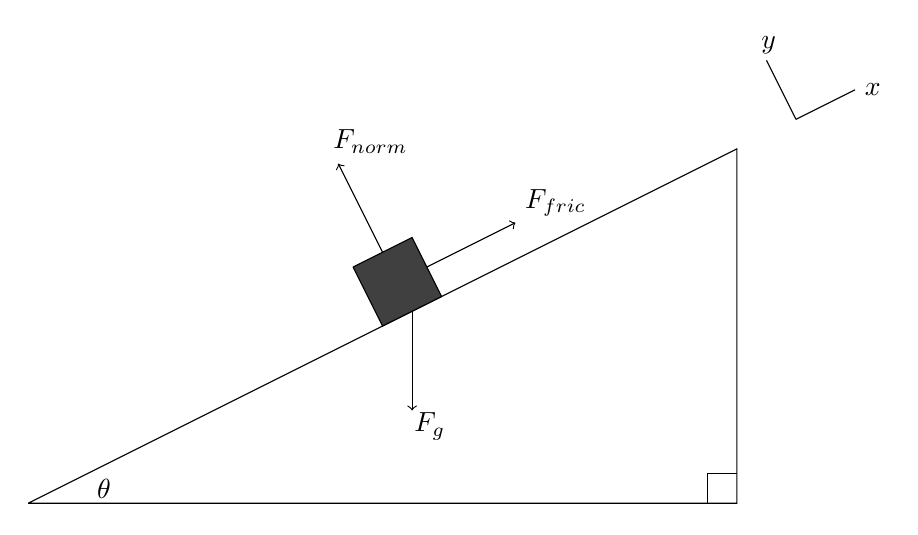
\begin{tikzpicture}
\draw[black] (0*0.75,0) -- (12*0.75,6*0.75) -- (12*0.75,0*0.75) -- (0*0.75,0*0.75);
\filldraw[draw = black, fill = darkgray] (5.5*0.75,4*0.75)--(6*0.75,3*0.75) -- (7*0.75,3.5*0.75) -- (6.5*0.75,4.5*0.75) -- (5.5*0.75, 4*0.75);
\draw[black] (1*0.75,0.25*0.75) node[anchor=west] {$\theta$};
\draw[black] (12*0.75,0.5*0.75) -- (11.5*0.75,0.5*0.75) -- (11.5*0.75,0*0.75);
\draw[->] (6.5*0.75,3.25*0.75) -- (6.5*0.75,1.57*0.75);
\draw[black] (6.375*0.75,1.3*0.75) node[anchor=west] {$F_g$};
\draw[->] (6.75*0.75,4*0.75) -- (8.25*0.75,4.75*0.75);
\draw[black] (8.25*0.75,4.75*0.75+0.25) node[anchor=west] {$F_{fric}$};
\draw[->] (6*0.75,4.25*0.75) -- (5.25*0.75,5.75*0.75);
\draw[black] (5*0.75,6.125*0.75) node[anchor=west] {$F_{norm}$};
\draw[black] (13*0.75,6.5*0.75) -- (14*0.75,7*0.75);
\draw[black](14*0.75,7*0.75) node[anchor=west] {$x$};
\draw[black] (13*0.75,6.5*0.75) -- (12.5*0.75,7.5*0.75);
\draw[black] (12.25*0.75,7.75*0.75) node[anchor=west] {$y$};

\end{tikzpicture}
\begin{center} 
(Fig. 3.5.1)
\end{center}
There are a countless number of dynamics problems that are out there and many of them you will be tested on. The classic ones are problems relating to objects going down ramps, being attached to springs, and being pulled by pulleys. We will go through some of these examples here and present a few other ideas. Fig. 3.5.1. depicts a drawing of a block that has been placed onto a ramp at an angle theta. There are a few things to note here. The first is that the force of gravity points directly down. This makes sense because we can assume the ramp is being placed flatly on earth. Next, we note the force of friction. It is pointing up, and this should be intuitive as we can assume that the block is currently moving down the ramp. Friction, as you know in your daily life, opposes the direction of motion. For now, that is all you need to know. Because the block is going down the ramp, the force points in the exact opposite direction of the motion. The last thing to note here is the direction of the Normal force. In the examples we have seen before, the Normal force is directly opposing the force of gravity, but this is not the case here. Here the normal force is directed perpendicular to the surface of the ramp. This is the nature of the Normal force. The Normal force will always point directly perpendicular to the surface area at which the block and the surface under the block(in this case the ramp) intersect. So if the ramp were completely horizontal, the force would point directly upward and if the ramp was completely vertical. The normal force would be completely horizontal. I like to conceptualize the normal force by imagining, in this case, that the ramp is to be made out of memory foam. If this was the case, the block would slightly come into the memory foam and deforms it. I like to think about the normal force as being the thing preventing this from happening at all(there still is a normal force in the case of memory foam, but it is different than in the case of the wooden block. Now that we are armed with these facts we will use some facts from trigonometry and Newton's laws to determine the motion of the block. We have to use trigonometry here because the forces are not directly perpendicular to each other, such that we can consider them to be acting in entirely different directions, or directly parallel, in which case we can use vector addition. The first thing we have to do is notice that the force of friction and the normal force are perpendicular to each other. This is helpful because we can keep us from having some trouble if we define the direction in which the friction acts(and also the direction of acceleration of the block as being the x-axis and the direction of the normal force as being the y-axis. Now we have to find the components of the force of gravity in the x and y directions. 
\newline
\newline
\newline
\begin{tikzpicture}
\draw[black] (0,0) -- (12,6) -- (12,0) -- (0,0);
\draw[black] (1,0) arc (0:28:1);
\draw[black] (1,0.25) node[anchor=west] {$\theta$};
\draw[black] (6.5,3.25) -- (6.5,0);
\draw[black] (12,0.5) -- (11.5,0.5) -- (11.5,0);
\draw[black] (6.5,0) -- (5.2,2.6);
\draw[black] (5.2,2.6) -- (5.4,2.7) -- (5.5,2.5) -- (5.3,2.4)    --(5.2,2.6);
\end{tikzpicture}
\begin{center} 
(Fig. 3.5.2)
\end{center}
As we can see in Fig. 3.5.2. We can draw a set of three triangles that will allow us to determine the $x$ and  $y$ components of the gravitational force. I will leave it as an exercise to the reader to find these components because it comes up very frequently and is a simple enough application of trigonometry that you should be able to find it on your own. However, as a disclaimer, it is a bit difficult. I will take the result that
\begin{equation}F_{g,x}=F_{g}\sin\left(\theta \right)\end{equation} and likewise \begin{equation}F_{g,y}=F_{g}\cos\left(\theta\right)\end{equation} Armed with these facts, we can now find the motion of the block. The first thing we have to realize is that we can separate $\vec{F}=m\vec{a}$ into the x and y directions such that $F_x=ma_x$. And  $F_y=ma_y$.  So we have \begin{equation}F_x= F_{g}\sin\left(\theta\right)-F_{friction}\end{equation} using the fact that the force of gravity in the x-direction is in the positive x-direction and the force of friction is in the -x-direction. We also have that \begin{equation}F_y=F_{normal}-F_{g}cos\left(\theta\right)\end{equation} Now that we have used Newton's laws, we have to use our physical insight to solve the rest of the problem. Just using the facts we have so far would not be enough to solve the problem. We have to recognize that the force in the y-direction must be 0 because the acceleration in the y-direction is 0. Think about this for a few seconds. Look at how we have defined the y-axis; this should make sense. The object is moving directly along the x-axis here; there is no y-motion. This is only counter-intuitive at first because we are used to thinking that if there is a downward motion, then there must be a y-acceleration. Of course, we have defined the y-axis differently here so this is not the case. Now we have that \begin{equation}0=F_{normal}-F_{g}cos\left(\theta\right)\end{equation} But the force of gravity is just $mg$ so we have that $$F_{normal}=mgcos\left(\theta\right)$$ Now we have to use Newton’s laws in the x-direction. We have that  $$F_x=F_{g}\sin\left(\theta \right)-F_{friction}$$ We know that the Force of gravity is just $mg$ and that $F_x=ma$. I am just writing $a$ here because of $a_y=0$. So $$ma=mg\sin\left(\theta \right)-F_{friction}$$ We can take $\mu$, the coefficient of friction, as a constant that is given to us. So we have that $$ma=mg\sin\left(\theta \right)-\mu F_{normal}$$ And that $$F_{normal}=mgcos\left(\theta \right)$$ If we multiply both sides of this second equation by $\mu$ we have that $$\mu F_{normal}=\mu mg\cos\left(\theta \right)$$ We can plug this new result into our first equation. We have that \begin{equation}ma=mg\sin\left(\theta \right)-\mu mgcos\left(\theta \right)\end{equation} We can cancel the mass out and factor out the $g$ to find that \begin{equation}a=g\left(\sin\left(\theta \right)-\mu cos\left(\theta \right)\right)\end{equation}Often times once we find out a result like this we need to test at edge cases where we can use our intuition to verify the result. This is necessary to verify that our equation is correct, although it does not prove that it is correct. If we say that $\theta=90^o $. We have that $a=g\left(1-\mu \theta \right)$. This means that $a=g$. This should be intuitive to us. If $\theta=90^o$ we have a completely vertical ramp, so the block is just undergoing free fall while next to the ramp. I encourage you to go through this example again because problems relating to ramps occur very frequently on the AP exam. 